\ATTR{[Last edit: Sept, 2022]}
%%%%%%%%%%%%%%%%%%%%%%%%%%%%%%%%%%%%%%%%%%%%%%%%%%%%%%%%%%%%%%%%%%%%%%%%%%%%%%%%
%% ************************************************************************** %%
%% *                                ABSTRACT.                               * %%
%% ************************************************************************** %%
%%%%%%%%%%%%%%%%%%%%%%%%%%%%%%%%%%%%%%%%%%%%%%%%%%%%%%%%%%%%%%%%%%%%%%%%%%%%%%%%
\begin{abstract}
This document describes the most common article elements and how to use the IEEEtran class with \LaTeX \ to produce files that are suitable for submission to the Institute of Electrical and Electronics Engineers (IEEE).  IEEEtran can produce conference, journal and technical note (correspondence) papers with a suitable choice of class options.
\end{abstract}

\begin{IEEEkeywords}
Class, IEEEtran, \LaTeX, paper, style, template, typesetting.
\end{IEEEkeywords}


%%%%%%%%%%%%%%%%%%%%%%%%%%%%%%%%%%%%%%%%%%%%%%%%%%%%%%%%%%%%%%%%%%%%%%%%%%%%%%%%
%% ************************************************************************** %%
%% *                            I - INTRO.                                  * %%
%% ************************************************************************** %%
%%%%%%%%%%%%%%%%%%%%%%%%%%%%%%%%%%%%%%%%%%%%%%%%%%%%%%%%%%%%%%%%%%%%%%%%%%%%%%%%
\section{Introduction}
\IEEEPARstart{I}{ntroduduction} starts here

%%%%%%%%% ========== [Definitions] ========== %%%%%%%%%
\subsection{Definitions}
Here, we will define \cite{FrictionPreferredGrasp} as in \Cref{fig:1}.
%% - FIG -- BEGIN --------------- %% [
\begin{figure}[h]
    \centering
    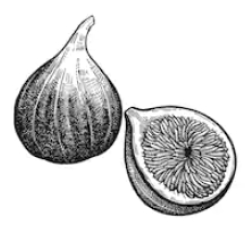
\includegraphics[width=2in]{Figs/fig1}
    \caption{A Caption}
    \label{fig:1}
\end{figure}
%% - FIG -- END ----------------- %% ]

\subsubsection{Levels}
%% - ENUM -- BEGIN --------------- %% [
\begin{enumerate}[label=\textbf{Level.\arabic*}]
    \item ABC \label{level:grasp:1}
    \item Something\label{level:grasp:2} 
    \item Repeat \label{level:grasp:3} \ref{level:grasp:2}
\end{enumerate}
%% - ENUM -- END ----------------- %% ]


%%%%%%%%%%%%%%%%%%%%%%%%%%%%%%%%%%%%%%%%%%%%%%%%%%%%%%%%%%%%%%%%%%%%%%%%%%%%%%%%
%% ************************************************************************** %%
%% *                            II - MOTIVATION                              * %%dd
%% ************************************************************************** %%
%%%%%%%%%%%%%%%%%%%%%%%%%%%%%%%%%%%%%%%%%%%%%%%%%%%%%%%%%%%%%%%%%%%%%%%%%%%%%%%%
\section{Motivation}
\noindent 


%%%%%%%%%%%%%%%%%%%%%%%%%%%%%%%%%%%%%%%%%%%%%%%%%%%%%%%%%%%%%%%%%%%%%%%%%%%%%%%%
%% ************************************************************************** %%
%% *                          III - BACKGROUND                              * %%
%% ************************************************************************** %%
%%%%%%%%%%%%%%%%%%%%%%%%%%%%%%%%%%%%%%%%%%%%%%%%%%%%%%%%%%%%%%%%%%%%%%%%%%%%%%%%
\section{Background}
\noindent \TODO{Here we will write about backgrounds}

%%%%%%%%% ========== [Visual Grasping] ========== %%%%%%%%%
\subsection{Types of visual grasping}
\TODO{surveys on different types of grasping approacches} 
\subsubsection{6-D pose grasping}
%%%%%%%%% ========== [SLAM] ========== %%%%%%%%%
\subsection{\gls{SLAM}}
\subsubsection{Kimera}

%%%%%%%%%%%%%%%%%%%%%%%%%%%%%%%%%%%%%%%%%%%%%%%%%%%%%%%%%%%%%%%%%%%%%%%%%%%%%%%%
%% ************************************************************************** %%
%% *                          IV - OUR METHODS                              * %%
%% ************************************************************************** %%
%%%%%%%%%%%%%%%%%%%%%%%%%%%%%%%%%%%%%%%%%%%%%%%%%%%%%%%%%%%%%%%%%%%%%%%%%%%%%%%%
\section{Our Methods}

%%%%%%%%% ========== [Concept] ========== %%%%%%%%%
\subsection{Conceptual Architecture}
\subsubsection{Problem Definition and Input Space}


\begin{equation}
  \hat{\xi} = \matb{\hatw & v \\ 0 & 0}, \quad 
    \hatw = \matb{\omega_1 \\ \omega_2 \\ \omega_3 }^{\wedge} = \matb{0 & -\omega_3 & \omega_2 \\ \omega_3 & 0 & -\omega_1 \\ -\omega_2 & \omega_1 & 0}
\end{equation}

%%%%%%%%%%%%%%%%%%%%%%%%%%%%%%%%%%%%%%%%%%%%%%%%%%%%%%%%%%%%%%%%%%%%%%%%%%%%%%%%
%% ************************************************************************** %%
%% *                         V - IMPLEMENTATION                             * %%
%% ************************************************************************** %%
%%%%%%%%%%%%%%%%%%%%%%%%%%%%%%%%%%%%%%%%%%%%%%%%%%%%%%%%%%%%%%%%%%%%%%%%%%%%%%%%
\section{Implementation}
